%versi 3 (22-07-2020)
\chapter{Landasan Teori}
\label{chap:teori}

\section{SharIF Judge}
\label{sec:judge}

SharIF Judge merupakan sebuah \textit{Online Judge} yang diambil dari Mohammed Javad Naderi yang dibentuk menggunakan CodeIgniter 3 dan diubah sesuai dengan kebutuhan di Informatika Universitas Katolik Parahyangan. SharIF Judge dapat menilai kode berbahasa \textit{C, C++, Java, dan Python} dengan mengunggah file ataupun mengetiknya langsung.

\subsection{Instalasi}

Berikut merupakan persyaratan dan langkah-langkah melakukan \textit{instalasi SharIF Judge}:

\subsubsection{Persyaratan}
SharIF Judge dapat dijalankan pada sistem operasi \textit{Linux} dengan syarat sebagai berikut:
\begin{itemize}
\item Diperlukan \textit{webserver} dengan versi PHP 5.3 atau lebih baru.
\item Pengguna dapat menjalankan PHP pada \textit{command line}. Pada \textit{Ubuntu} diperlukan instalasi paket \textit{php5-cli}.
\item \textit{MySql database} dengan ekstensi \textit{Mysqli} untuk PHP atau \textit{PostgreSql database}.
\item PHP harus memiliki akses untuk menjalankan perintah melalui fungsi \textit{shell\textunderscore exec}.

\begin{lstlisting}[language=Java, caption=Kode untuk melakukah pengetesan fungsi \textit{shell_exec}, label=kode:shell]
	echo shell_exec("php -v");
\end{lstlisting}

\item \textit{Tools} untuk melakukan kompilasi dan menjalankan kode yang dikumpulkan (\textit{gcc, g++, javac, java, python2, python3}).
\item \textit{Perl} disarankan untuk diinstalasi untuk alasan ketepatan waktu, batas memori, dan memaksimalkan batas ukuran pada hasil kode yang dikirim.
\end{itemize}

\subsubsection{Instalasi}
\begin{itemize}
\item Mengunduh versi terakhir dari \textit{SharIF Judge} dan melakukan \textit{unpack} pada direktori \textit{public html}.
\item Memindahkan \textit{folder system} dan \textit{application} diluar direktori \textit{public} dan mengubah \textit{path} pada \verb|index.php|(Opsional).
\begin{lstlisting}[language=Java, caption=Contoh \textit{path} pada halaman index.php, label=kode:movesystemandapp]
	$system_path = '/home/mohammad/secret/system';
	application_folder = '/home/mohammad/secret/application';
\end{lstlisting}
\item Membentuk \textit{database MySql} atau \textit{PostgreSql} untuk \textit{SharIF Judge}. Jangan melakukan instalasi paket koneksi \textit{database} apapun untuk \textit{C, C++, Java,} atau \textit{Python}.

\end{itemize}

\subsection{\textit{Clean Urls}}


\subsection{Users}
\subsection{Menambah Assignment}
\subsection{Sample Assignment}

\section{CodeIgniter 3}
\label{sec:ci3} 
 
CodeIgniter 3 merupakan sebuah \textit{framework} yang berfungsi untuk mempermudah penggunanya dalam membentuk aplikasi \textit{website} menggunakan bahasa PHP. CodeIgniter 3 menggunakan struktur MVC (dapat dilihat pada Gambar ~\ref{fig:mvc})) dalam pembentukan \textit{website}.
\begin{figure}[H]
	\centering  
	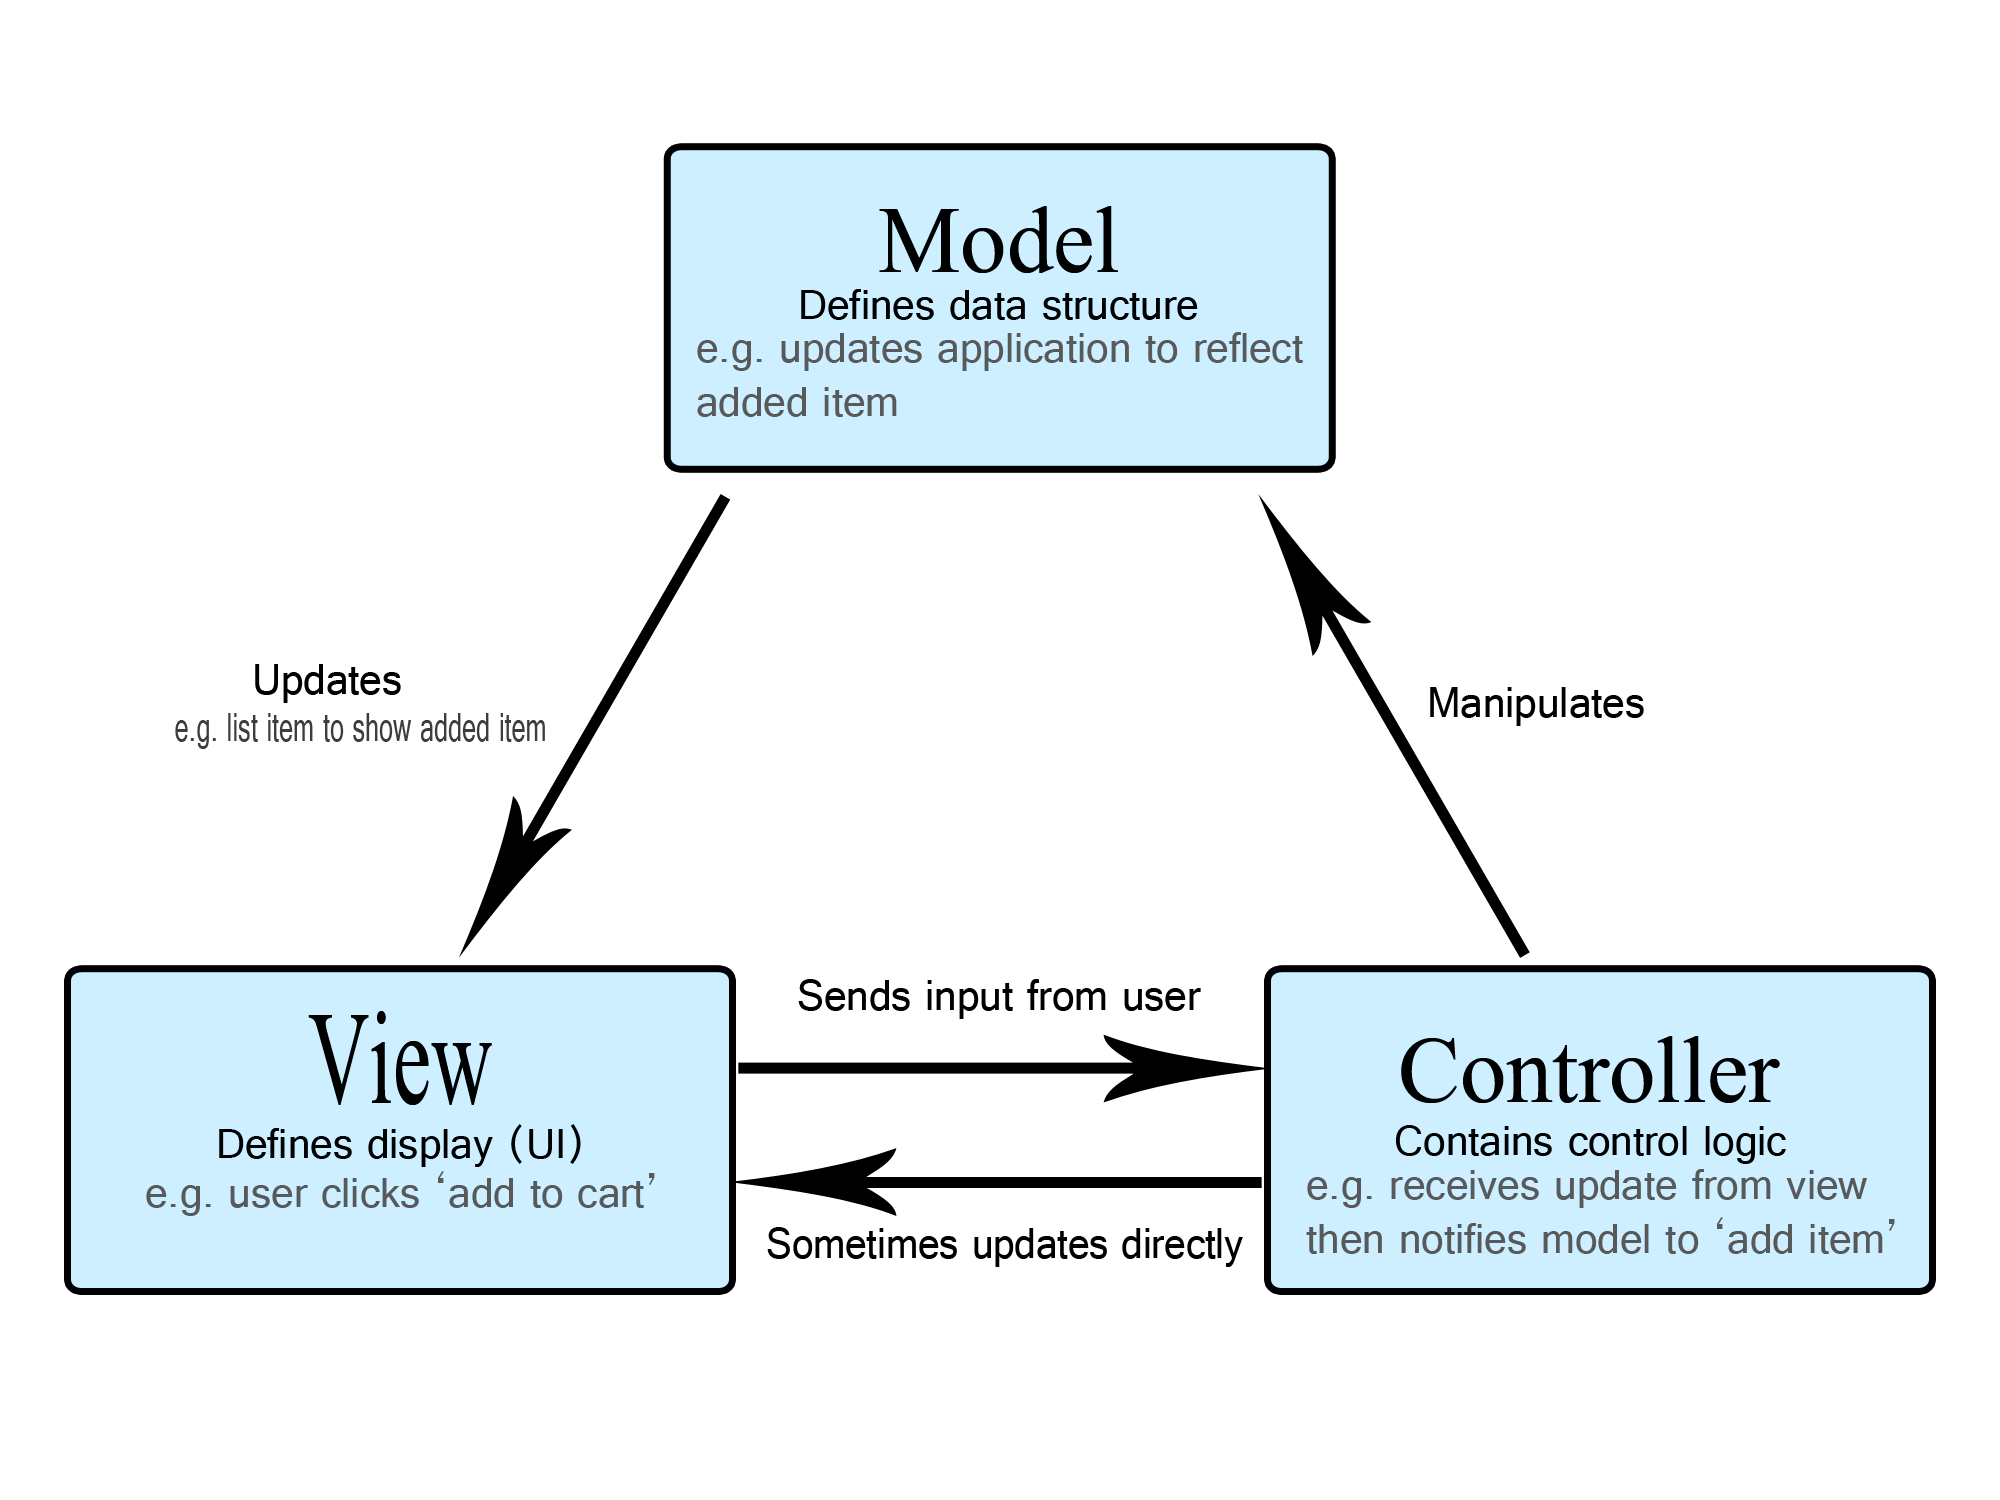
\includegraphics[scale=0.5]{mvc}  
	\caption[Gambar arsitektur MVC]{Gambar arsitektur MVC} 
	\label{fig:mvc} 
\end{figure} 

MVC membagi struktur \textit{folder} menjadi 3 buah dengan fungsi berbeda yaitu Model, View, Controller. Model

\section{CodeIgniter 4}
\label{sec:ci4}

CodeIgniter 4 merupakan versi terbaru dari \textit{framework} CodeIgniter.


\section{Koversi CodeIgniter 3 ke CodeIgniter 4 \footnote{\url{https://codeigniter.com/user_guide/installation/upgrade_4xx.html}}}
\label{sec:konversici3c4}
 
CodeIgniter 3 sedang mengalami fase \textit{maintenance} sehingga perlu dilakukan konversi menjadi CodeIgniter 4. Konversi CodeIgniter 3 ke CodeIgniter 4 diperlukan penulisan ulang karena terdapat banyak implementasi yang berbeda. Konversi ke CodeIgniter 4 diawali dengan melakukan instalasi projek baru CodeIgniter 4.


\subsection{Struktur Aplikasi}

Struktur direktori pada CodeIgniter 4 memiliki perubahan yang terdiri \textit{app, public, dan writable}. Direktori app merupakan perubahan dari direktori application dengan isi yang hampir sama dengan beberapa perubahan nama dan perpindahan direktori. Pada CodeIgniter 4 terdapat direktori \textit{public} yang bertujuan sebagai direktori utama pada aplikasi website. Selanjutnya terdapat direktori \textit{writable} yang berisikan \textit{cache data, logs,} dan \textit{session data}.


\textbf{\textit{Routing}}

CodeIgniter 4 meletakan \textit{route} pada \textit{file} \verb|app\Config\Routes.php|. CodeIgniter 4 memiliki fitur \textit{auto routing} seperti pada CodeIgniter 3 namun, pada \textit{default} di matikan. Fitur \textit{auto routing} memungkinkan untuk dinyalakan serupa dengan pada CodeIgniter 3 namun tidak direkomendasikan karena alasan \textit{security}.  
 
 
\textbf{\textit{Model, View, and Controller}}
 
Struktur MVC pada CodeIgniter 4 berbeda dibandingkan CodeIgniter 3 dimana pada CodeIgniter 4 direktori \textit{Model} terdapat pada direktori \verb|app\Models|. Pembentukan \textit{file} untuk \textit{Model} perlu ditambahkan \verb|namespace App\Models;| dan \verb|use CodeIgniter\Model;| pada awal \textit{file} setelah membuka tag PHP. Selanjutnya nama fungsi perlu diubah dari \verb|extends CI_Model| menjadi \verb|extends Model|. 
 
\textit{View} pada CodeIgniter 4 terdapat di \verb|app\Views| dengan sintaks yang harus diubah. Sintaks yang harus diubah merupakan sintaks untuk memanggil \textit{view} pada CodeIgniter 3 \verb|$this->load->view('x');| sedangkan pada CodeIgniter 4 dapat menggunakan \verb|return view('x);|. Selanjutnya, sintaks \verb|<?php echo $title?>| pada halaman \textit{view} dapat diubah menjadi
 \verb|<?= $title ?>|. 
 
\textit{Controller} pada CodeIgniter 4 terdapat di \verb|app\Controllers| dan diperlukan beberapa perubahan. Pertama, perlu ditambahkan \verb|namespace App\Controllers;| pada awal \textit{file} setelah membuka tag PHP. Selanjutnya, perlu mengubah \verb|extends CI_Controller| menjadi \verb|extends BaseController|. Selanjutnya, diperlukan pengubahan nama pada pemanggilan \textit{file} menjadi \verb|App\Controllers\User.php| .
 
\textbf{\textit{Libraries}}
 
CodeIgniter 4 menyediakan \textit{library} untuk digunakan dan dapat diinstall apabila diperlukan. Pemanggilan \textit{library} berubah dari \verb|$this->load->library('x');| menjadi \verb|$this->x = new X();|. Terdapat beberapa \textit{library} yang harus di \textit{upgrade} dengan sedikit perubahan.
 

\textbf{\textit{Helpers}}
 
\textit{Helpers} tidak terdapat banyak perubahan namun, beberapa \textit{helpers} pada \textit{CodeIgniter 3} tidak terdapat pada \textit{CodeIgniter 4} sehingga perlu perubahan pada implementasi fungsinya. \textit{Helpers} dapat di dimuat secara otomatis menggunakan \verb|app\Config\Autoload.php|


\textbf{\textit{Events}}


\textbf{\textit{Framework}}


\textbf{\textit{Configuration}}

\textit{File configuration} CodeIgniter 4 terdapat pada \verb|app\Config| dengan penulisan sedikit berbeda dengan versi sebelumnya. Pengguna hanya perlu melakukan pemindahan menuju CodeIgniter 4 dan apabila menggunakan \textit{file config custom} maka, diperlukan penulisan ulang pada direktori Config dengan melakukan \textit{extend} pada \verb|CodeIgniter\Config\BaseConfig|.   

\textbf{\textit{Database}}

Penggunaan \textit{database} pada CodeIgniter 4 hanya berubah sedikit dibandingkan dengan versi sebelumnya. Data-data penting kredensial diletakan pada \verb|app\Config\Database.php| dan perlu dilakukan beberapa perubahan sintaks dan \textit{query}. Sintaks untuk memuat database diubah menjadi \verb|$db = db_connect();| dan  apabila menggunakan beberapa \textit{database} maka sintaks menjadi \verb|$db = db_connect('group_name');|. Semua \textit{query} harus diubah dari \verb|$this->db| menjadi \verb|$db| dan beberapa sintaks perlu diubah seperti \verb|$query->result();| menjadi \verb|$query->getResult();|. Selain itu, terdapat \textit{class} baru yakni \textit{Query Builder Class} yang harus di inisiasi \verb|$builder = $db->table('mytable');| dan dapat dipakai untuk menjalankan \textit{query} dengan mengganti \verb|$this->db| seperti \verb|$this->db->get();| menjadi \verb|$builder->get();|.

\textbf{\textit{Emails}}

Perubahan \textit{email} hanya terdapat pada nama dari \textit{method} dan pemanggilan \textit{library email}. Pemanggilan  \textit{library} berubah dari \verb|$this->load->library('email);| menjadi \verb|$email = service('email');| dan selanjutnya perlu dilakukan perubahan pada semua \verb|$this->email| menjadi \verb|$email|. Selanjutnya beberapa pemanggilan \textit{method} berubah dengan tambahan \textit{set} didepannya seperti \textit{from} menjadi \textit{setFrom}.

\textbf{\textit{Encryption}}

Terdapat perubahan 

\textbf{\textit{Working with Uploaded Files}}

Terdapat banyak perubahan dimana pada CodeIgniter 4 pengguna dapat mengecek apakah \textit{file} telah terunggah tanpa \textit{error} dan lebih mudah untuk melakukan penyimpanan \textit{file}. Pada CodeIgniter 4 melakukan akses pada \textit{uploaded file} dilakukan dengan \verb|$file = $this->request->getFile('userfile')| dan dapat dilakukan validasi dengan cara \verb|$file->isValid()|. Penyimpanan \textit{file} yang sudah diunggah dapat dilakukan dengan \verb|$path = $this->request->getFile('userfile')->store('head_img/', 'user_name.jpg');|. \textit{File} yang sudah diunggah dan di validasi akan tersimpan pada \verb|writable/uploads/head_img/user_name.jpg.|

\textbf{\textit{HTML Tables}}

Tidak terdapat banyak perubahan pada \textit{framework} versi terbaru hanya perubahan pada nama \textit{method} dan pemanggilan \textit{library}. Perubahan pemanggilan \textit{library} dari \verb|$this->load->library('table');| menjadi \verb|$table = new \CodeIgniter\View\Table();| dan perlu dilakukan perubahan setiap \verb|$this->table| menjadi \verb|$table|. Selain itu, terdapat bebera perubahan pada penamaan \textit{method} dari \textit{underscored} menjadi \textit{camelCase}.


\textbf{\textit{Localization}}

\textit{CodeIgniter 4} mengembalikan \textit{file} bahasa menjadi \textit{array} sehingga perlu dilakukan beberapa perubahan. Pertama, perlu dilakukan konfigurasi \textit{default languange} 
pada perangkat lunak. Selanjutnya melakukan pemindahan \textit{file} bahasa pada \textit{CodeIgniter 3} menuju \verb|app\Languange\<locale>|. \textit{File-file} bahasa \textit{CodeIgniter 3} perlu dilakukan penghapusan semua kode \verb|$this->lang->load($file, $lang);| dan mengubah \textit{method} pemanggilan bahasa dari \verb|$this->lang->line('error_email_missing')| menjadi \verb|echo lang('Errors.errorEmailMissing');|
 
\textbf{\textit{Migrations}}

Perubahan perlu dilakukan pada nama \textit{file} menjadi nama dengan cap waktu. Selanjutnya dilakukan penghapusan kode \verb|defined('BASEPATH') OR exit('No direct script access allowed');| dan menambahkan dua buah kode yakni, \verb|namespace App\Database\Migrations;| dan \verb|use CodeIgniter\Database\Migration;| setelah membuka tag PHP. Setelah itu, \verb|extends CI_Migration| diubah menjadi \verb|extends Migration|. Terakhir, terdapat perubahan pada nama \textit{method} \textit{Forge} dari \verb|$this->dbforge->add_field| menjadi \textit{camelCase} \verb|$this->forge->addField|.
 
\textbf{\textit{Pagination}}



\textbf{\textit{HTTP Response}}



\textbf{\textit{Routing}}



\textbf{\textit{Security}}



\textbf{\textit{Sessions}}



\textbf{\textit{Validations}}



\textbf{\textit{View Parser}}


\subsection{Tabel}  
Berikut adalah contoh pembuatan tabel. 
Penempatan tabel dan gambar secara umum diatur secara otomatis oleh \LaTeX{}, perhatikan contoh di file bab2.tex untuk melihat bagaimana cara memaksa tabel ditempatkan sesuai keinginan kita.

Perhatikan bawa berbeda dengan penempatan judul gambar gambar, keterangan tabel harus diletakkan di atas tabel!!
Lihat Tabel~\ref{tab:contoh1} berikut ini:

\begin{table}[H] %atau h saja untuk "kira kira di sini"
	\centering 
	\caption{Tabel contoh}
	\label{tab:contoh1}
	\begin{tabular}{cccc}
		\toprule
		& $v_{start}$ & $\mathcal{S}_{1}$ & $v_{end}$\\

		\midrule
		$\tau_{1}$ & 1 & 12& 20\\
		$\tau_{2}$ & 1 &  & 20\\
		$\tau_{3}$ & 1 & 9 & 20\\
		$\tau_{4}$ & 1 &  & 20\\

		\bottomrule
		
	\end{tabular} 
\end{table}
Tabel~\ref{tab:cthwarna1} dan Tabel~\ref{tab:cthwarna2} berikut ini adalah tabel dengan sel yang berwarna dan ada dua tabel yang bersebelahan. 
\begin{table}[H]
	\begin{minipage}[c]{0.49\linewidth}
		\centering
		\caption{Tabel bewarna(1)}
		\label{tab:cthwarna1}
		\begin{tabular}{ccccc}
			\toprule
			 & $v_{start}$ & $\mathcal{S}_{2}$ & $\mathcal{S}_{1}$ & $v_{end}$\\
			
			\midrule
			$\tau_{1}$ & 1 & 5 \cellcolor{green}& 12& 20\\
			$\tau_{2}$ & 1 & 8 \cellcolor{green}& & 20\\
			$\tau_{3}$ & 1 & 2/8/17 \cellcolor{green}& 9 & 20\\
			$\tau_{4}$ & 1 & \cellcolor{red}& & 20\\
			
			\bottomrule

		\end{tabular}
	\end{minipage}
	\begin{minipage}[c]{0.49\linewidth}
		
		\centering 
		\caption{Tabel bewarna(2)}
		\label{tab:cthwarna2}
		\begin{tabular}{ccccc}
			\toprule
			 & $v_{start}$ & $\mathcal{S}_{1}$ & $\mathcal{S}_{2}$ & $v_{end}$\\
			
			\midrule
			$\tau_{1}$ & 1 & 12& 5 \cellcolor{red} &20\\
			$\tau_{2}$ & 1 &  &  8 \cellcolor{green} &20\\
			$\tau_{3}$ & 1 & 9 & 2/8/17 \cellcolor{green} &20\\
			$\tau_{4}$ & 1 &   & \cellcolor{red} &20\\
			
			\bottomrule
		
		\end{tabular}
	\end{minipage}
\end{table}

 
\subsection{Kutipan}
\label{subs:kutipan} 
Berikut contoh kutipan dari berbagai sumber, untuk keterangan lebih lengkap, silahkan membaca file referensi.bib yang disediakan juga di template ini.
Contoh kutipan:
\begin{itemize}
	\item Buku:~\cite{berg:08:compgeom} 
	\item Bab dalam buku:~\cite{kreveld:04:GIS}
	\item Artikel dari Jurnal:~\cite{buchin:13:median}
	\item Artikel dari prosiding seminar/konferensi:~\cite{kreveld:11:median}
	\item Skripsi/Thesis/Disertasi:~\cite{lionov:02:animasi}~\cite{wiratma:10:following}~\cite{wiratma:22:later}
	\item Technical/Scientific Report:~\cite{kreveld:07:watertight}
	\item RFC (Request For Comments):~\cite{RFC1654}
	\item Technical Documentation/Technical Manual:~\cite{Z.500}~\cite{unicode:16:stdv9}~\cite{google:16:and7}
	\item Paten:~\cite{webb:12:comm}
	\item Tidak dipublikasikan:~\cite{wiratma:09:median}~\cite{lionov:11:cpoly}
	\item Laman web:~\cite{erickson:03:cgmodel}  
	\item Lain-lain:~\cite{agung:12:tango}
\end{itemize}    
  
\subsection{Gambar}

Pada hampir semua editor, penempatan gambar di dalam dokumen \LaTeX{} tidak dapat dilakukan melalui proses {\it drag and drop}.
Perhatikan contoh pada file bab2.tex untuk melihat bagaimana cara menempatkan gambar.
Beberapa hal yang harus diperhatikan pada saat menempatkan gambar:
\begin{itemize}
	\item Setiap gambar {\bf harus} diacu di dalam teks (gunakan {\it field} {\sc label})
	\item {\it Field} {\sc caption} digunakan untuk teks pengantar pada gambar. Terdapat dua bagian yaitu yang ada di antara tanda $[$ dan $]$ dan yang ada di antara tanda $\{$ dan $\}$. Yang pertama akan muncul di Daftar Gambar, sedangkan yang kedua akan muncul di teks pengantar gambar. Untuk skripsi ini, samakan isi keduanya.
	\item Jenis file yang dapat digunakan sebagai gambar cukup banyak, tetapi yang paling populer adalah tipe {\sc png} (lihat Gambar~\ref{fig:ularpng}), tipe {\sc jpg} (Gambar~\ref{fig:ularjpg}) dan tipe {\sc pdf} (Gambar~\ref{fig:ularpdf})
	\item Besarnya gambar dapat diatur dengan {\it field} {\sc scale}.
	\item Penempatan gambar diatur menggunakan {\it placement specifier} (di antara tanda  $[$ dan $]$ setelah deklarasi gambar.
	Yang umum digunakan adalah {\bf H} untuk menempatkan gambar {\bf sesuai} penempatannya di file .tex atau  {\bf h} yang berarti "kira-kira" di sini. \\
	Jika tidak menggunakan {\it placement specifier}, \LaTeX{} akan menempatkan gambar secara otomatis untuk menghindari bagian kosong pada dokumen anda.
	Walaupun cara ini sangat mudah, hindarkan terjadinya penempatan dua gambar secara berurutan. 	
	\begin{itemize}
		\item Gambar~\ref{fig:ularpng} ditempatkan di bagian atas halaman, walaupun penempatannya dilakukan setelah penulisan 3 paragraf setelah penjelasan ini.
		\item Gambar~\ref{fig:ularjpg} dengan skala 0.5 ditempatkan di antara dua buah paragraf. Perhatikan penulisannya di dalam file bab2.tex!
		\item Gambar~\ref{fig:ularpdf} ditempatkan menggunakan {\it specifier} {\bf h}.
	\end{itemize}
\end{itemize}
 
\dtext{17-18}
\begin{figure} 
	\centering  
	\includegraphics[scale=1]{ular-png}  
	\caption[Gambar {\it Serpentes} dalam format png]{Gambar {\it Serpentes} dalam format png} 
	\label{fig:ularpng} 
\end{figure} 

\dtext{19-20}
\begin{figure}[H]
	\centering  
	\includegraphics[scale=0.5]{ular-jpg}  
	\caption[Ular kecil]{Ular kecil} 
	\label{fig:ularjpg} 
\end{figure} 
\dtext{21-22}

\begin{figure}[ht] 
	\centering  
	\includegraphics[scale=1]{ular-pdf}  
	\caption[ {\it Serpentes} betina]{ {\it Serpentes} jantan} 
	\label{fig:ularpdf} 
\end{figure} 
 
\subsection{Kode Program}

Kode program dalam bahasa tertentu seringkali harus ditulis di dalam bab, bukan hanya dilampirkan di bagian Lampiran. 
Kode~\ref{kode:aneh} menampilkan penggunaan karakter-karakter yang umum digunakan dalam sebuah program yang ditulis dengan bahasa C.


\begin{lstlisting}[language=Java, caption=Kode untuk menampilkan karakter-karakter aneh, label=kode:aneh]
// This does not make algorithmic sense, 
// but it shows off significant programming characters.

#include<stdio.h>

void myFunction( int input, float* output ) {
	switch ( array[i] ) {
		case 1: // This is silly code
			if ( a >= 0 || b <= 3 && c != x )
				*output += 0.005 + 20050;
			char = 'g';
			b = 2^n + ~right_size - leftSize * MAX_SIZE;
			c = (--aaa + &daa) / (bbb++ - ccc % 2 );
			strcpy(a,"hello $@?"); 
	}
	count = ~mask | 0x00FF00AA;
}

// Fonts for Displaying Program Code in LATEX
// Adrian P. Robson, nepsweb.co.uk
// 8 October 2012
// http://nepsweb.co.uk/docs/progfonts.pdf

\end{lstlisting}

\subsection{Notasi}

Simbol-simbol (matematika) yang sering digunakan sepanjang penulisan skripsi, dapat dimasukkan ke dalam ``Daftar Notasi''. Daftar ini ada di halaman depan sebelum Bab~\ref{chap:intro}.
Cara memasukkan sebuah simbol ke dalam Daftar Notasi adalah menggunakan perintah \verb|\nomenclature|. Contoh:
\begin{center}
    \verb|\nomenclature[]{$A$}{luas kandang ular}|    
\end{center}
\nomenclature[]{$A$}{luas kandang ular}
\nomenclature[]{$n$}{banyaknya ular}
\nomenclature[]{$k$}{jumlah kepala per seekor ular\nomrefpage}
Argumen opsional digunakan untuk mengurutkan notasi. Silahkan lihat sendiri dokumentasi package \verb|nomencl|

